%%%%%%%% Klassen-Optionen
\documentclass[12pt,a4paper]{scrartcl}

%%%%%%%% PAKETE: unverzichtbare Pakete mit Einstellungen
\usepackage[left=2.5cm, right=2cm, top=3cm, bottom=3cm, a4paper]{geometry} %Seitenrände
\usepackage[utf8x]{inputenc} % utf8-Kodierung und direkte Eingabe von Sonderzeichen
\usepackage{fixltx2e} % Verbessert einige Kernkompetenzen von LaTeX2e

%%%%%%%% PAKETE: AMS-Pakete
\usepackage{amsmath} % Mathe-Erweiterung
\usepackage{amsfonts} % Schrift-Erweiterung
\usepackage{amssymb} % Sonderzeichen-Erweiterung

%%%%%%%% PAKETE: Sonstiges
\usepackage[colorlinks, citecolor=black, filecolor=black, linkcolor=black, urlcolor=black]{hyperref} % Links
\usepackage{wrapfig} % ausgeklügekte Floatumgebung
\usepackage{float} % normale Floatumgebung
\restylefloat{figure} % ermöglicht die Verwendung von "H" (ist noch stärker als "h!")
\usepackage[small,it,singlelinecheck=false]{caption} % Bildunterschriften formatieren
\usepackage{multirow} % ermöglich Verbinden von Tabellenzeilen
\usepackage{multicol} % ermöglicht Spalten
\usepackage{fancyhdr} % ermöglicht Kopf- und Fußzeilen
\usepackage{graphicx} % Einbinden von Bildern möglich
\usepackage{units} % Einheiten
\usepackage{subcaption}

%%%%%%%% DEFINITIONEN: Titelseite
\author{April Cooper, Patrick Kreissl und Sebastian Weber}
\title{Worksheet 1: Quantum mechanical approaches:
Hückel approximation and DFT methods}
\publishers{University of Stuttgart}
\date{\today}

%%%%%%%% ANPASSUNGEN: Kopf-und Fußzeile
\fancypagestyle{plain}{} % redefine the plain pagestyle to match the fancy layout
\pagestyle{fancy} % aktiviere eigenen Seitenstil
\fancyhf{} % alle Kopf- und Fußzeilen bereinigen
\fancyhead[L]{Worksheet 1: Quantum mechanical approaches}
\fancyhead[R]{\today}
\renewcommand{\headrulewidth}{0.6pt} % obere Trennlinie
\fancyfoot[L]{April Cooper, Patrick Kreissl und Sebastian Weber}
\fancyfoot[R]{Page \thepage}
\renewcommand{\footrulewidth}{0.6pt} % untere Trennlinie

%%%%%%%% ANPASSUNGEN: Absätze
\setlength{\parindent}{0em} % keine Absatzeinzüge
\setlength{\parskip}{0.5em} % Absatz-Abstand

%%%%%%%% ANPASSUNGEN: Abbildungsverzeichnis
\usepackage{tocloft} % Zum Anpassen der Verzeichnisse
%\renewcommand{\cftfigpresnum}{Abb. }
%\renewcommand{\cfttabpresnum}{Tab. }
\renewcommand{\cftfigaftersnum}{:}
\renewcommand{\cfttabaftersnum}{:}
\setlength{\cftfignumwidth}{2cm}
\setlength{\cfttabnumwidth}{2cm}
\setlength{\cftfigindent}{0cm}
\setlength{\cfttabindent}{0cm}

%%%%%%%% SONSTIGES
\usepackage{pdfpages}
\usepackage{pgf}
%\usepackage{subfigure}
\usepackage{graphicx}
\usepackage{caption}
\usepackage{subcaption}

% NÜTZLICH: http://truben.no/latex/table/

% Anfang des eigentlichen Dokuments
\begin{document}

\maketitle
\tableofcontents
\newpage

% =============== Section ============
\section{Computational Task: DFT calculations with Siesta}

\subsection{Geometry optimization of adenine}

\begin{table}[H]
\begin{tabular}{c|c|c|c||c|c|c|c} 
Distance in \r{A} & GGA & LDA & Exp\footnotemark[1] & Angle in degrees & GGA & LDA  & Exp\footnotemark[1]\\ 
\hline 
\hline
C2-N3 & 1.353 & 1.338 & 1.332 & N3-C4-C5 & 127.37 & 127.17 & 126.9 \\ 
\hline 
N1-C2 & 1.357 & 1.343 & 1.338 & C2-N3-C4 & 110.51 & 111.13 & 110.8 \\ 
\hline 
C6-N1 & 1.356 & 1.342 & 1.349 & N9-C4-C5 & 104.16 & 104.16 & 105.7 \\ 
\hline 
C5-C6 & 1.427 & 1.415 & 1.409 & C8-N9-C4 & 106.94 & 107.01 & 105.9 \\ 
\hline 
C4-C5 & 1.415 & 1.406 & 1.382 & N7-C8-N9 & 113.51 & 113.28 & 113.8 \\ 
\hline 
N3-C4 & 1.351 & 1.336 & 1.342 & C5-N7-C8 & 103.60 & 103.88 & 103.9 \\  
\end{tabular} 
\caption{Bond lengths and bond angles predicted by siesta and experimental data.}\label{tab:distances_and_angles}
\end{table}

\footnotetext[1]{source: Attachment1a.pdf}

With both used methods (generalized gradient approximation GGA and local density approximation LDA) the results predicted by siesta are quite close to the experimental data (table \ref{tab:distances_and_angles}). In general for the bond lengths the with LDA predicted data is quite close to the experimental results while the GGA data always overestimate the bond lengths. \\
For nearly all predicted bond angles the GGA data is closer to the experiments than the LDA data. However the LDA results vary only a litte from the GGA results.\\
So from this little trial run it seem that if one is looking for bond lengths using LDA for predictions would be a better choice than using GGA. Also the predicted angles would be pretty close to the experimental data. For more accuracy computing the bond angles GGA would possibly be an even better choice.

\newpage

\subsection{Theoretical Prediction of Watson-Crick Hydrogen-bond length in
adenine-thymine base pair}

\begin{figure}[H]
        \centering
        \begin{subfigure}[b]{0.49\textwidth}
                \centering
                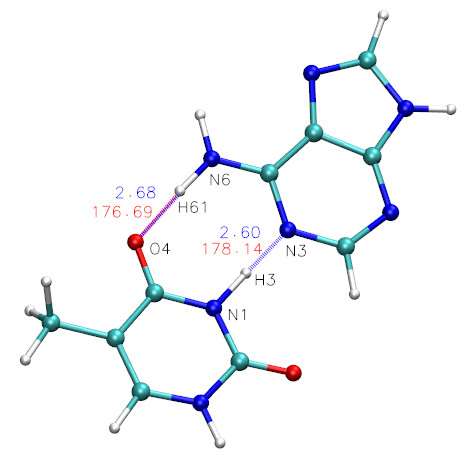
\includegraphics[width=\textwidth]{lda.jpg}
                \caption{LDA}
                \label{fig:gull}
        \end{subfigure}
        \begin{subfigure}[b]{0.49\textwidth}
                \centering
                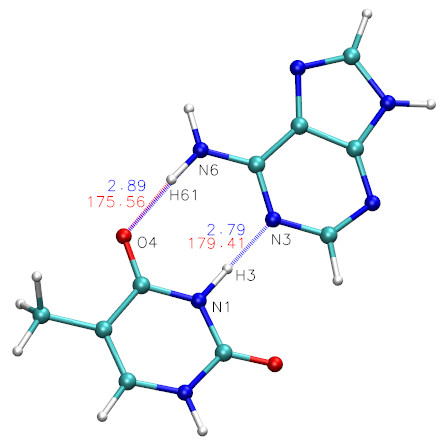
\includegraphics[width=\textwidth]{gga.jpg}
                \caption{GGA}
                \label{fig:tiger}
        \end{subfigure}
        \caption{Results for two flavours of XC functional. Blue numbers show bond lengths and red ones show bond angles.}\label{fig:ade-thy}
\end{figure}

\begin{table}[H]
\begin{tabular}{l||l|l|l}
Angle in degrees & LDA & GGA & Literature \footnotemark[2]\\ 
\hline \hline 
O4-H61-N6 & 176.7 & 175.6 & 175.8\\ 
\hline 
N1-H3-N3 & 178.1 & 179.4 & 178.1\\ 
\end{tabular}
\caption{Bond angles}\label{tab:angles}
\end{table}

\begin{table}[H]
\begin{tabular}{l||l|l|l|l}
Distance in \r{A} & LDA & GGA & Experiment 1 \footnotemark[2] & Experiment 2 \footnotemark[2] \\ 
\hline \hline 
O4-N6 & 2.68 & 2.89 & 2.95 & 2.93 \\ 
\hline 
N1-N3 & 2.60 & 2.79 & 2.82 & 2.85 \\ 
\end{tabular}
\caption{Bond lengths}\label{tab:lengths}
\end{table}

\footnotetext[2]{source: Attachment1b.pdf}

With LDA (local density approximation) and GGA (generalized gradient approximation) you get decent results. Both show that the O4-N6 bound is around $\unit[8 - 10]{\r{A}}$ longer than the N1-N3 bound. The comparison with experimental data (see table \ref{tab:lengths}) illustrates that GGA is more precise than LDA. For GGA the deviation is around $\unit[2]{\%}$ and for LDA around $\unit[10]{\%}$. However the exact error can't be specified because you don't have an isolated adenine-thymine base pair in the real world and the experimental results depend on the chemical environment.

The high precision of GGA can be explained by the fact that it uses the gradient which is non-local. In contrast LDA is a local approximation. It overestimates the bond strength regularly. Therefor the bond lengths are to short. LDA is highly precise only if you have a structure with uniform electron density.

The calculated bond angles are in conformity with calculated values that were found in Attachment1b.pdf (see Table \ref{tab:angles}). It's virtually impossible to figure out whether their calculation is more exact than ours.

For convergence GGA needed 64 steps and LDA 70 steps. A GGA step is more time consuming than a LDA step due to the use of the gradient. Therefore GGA ran for $\unit[52]{min}$ and LDA for $\unit[49]{min}$. As you can see the difference in run time is very small so that you should use GGA for all similar problems because of higher precision.

\end{document}


% =============== Comments ============
\begin{comment}
\verb{x_init {}}

\begin{figure}[H]
	\resizebox{1\textwidth}{!{\input{../plots/NAME.pgf}}
	\caption{CAPTION}\label{fig:NAME}
\end{figure}
\end{comment}
